\documentclass[twoside]{book}

% Packages required by doxygen
\usepackage{calc}
\usepackage{doxygen}
\usepackage{graphicx}
\usepackage[utf8]{inputenc}
\usepackage{makeidx}
\usepackage{multicol}
\usepackage{multirow}
\usepackage{textcomp}
\usepackage[table]{xcolor}

% Font selection
\usepackage[T1]{fontenc}
\usepackage{mathptmx}
\usepackage[scaled=.90]{helvet}
\usepackage{courier}
\usepackage{amssymb}
\usepackage{sectsty}
\renewcommand{\familydefault}{\sfdefault}
\allsectionsfont{%
  \fontseries{bc}\selectfont%
  \color{darkgray}%
}
\renewcommand{\DoxyLabelFont}{%
  \fontseries{bc}\selectfont%
  \color{darkgray}%
}

% Page & text layout
\usepackage{geometry}
\geometry{%
  a4paper,%
  top=2.5cm,%
  bottom=2.5cm,%
  left=2.5cm,%
  right=2.5cm%
}
\tolerance=750
\hfuzz=15pt
\hbadness=750
\setlength{\emergencystretch}{15pt}
\setlength{\parindent}{0cm}
\setlength{\parskip}{0.2cm}
\makeatletter
\renewcommand{\paragraph}{%
  \@startsection{paragraph}{4}{0ex}{-1.0ex}{1.0ex}{%
    \normalfont\normalsize\bfseries\SS@parafont%
  }%
}
\renewcommand{\subparagraph}{%
  \@startsection{subparagraph}{5}{0ex}{-1.0ex}{1.0ex}{%
    \normalfont\normalsize\bfseries\SS@subparafont%
  }%
}
\makeatother

% Headers & footers
\usepackage{fancyhdr}
\pagestyle{fancyplain}
\fancyhead[LE]{\fancyplain{}{\bfseries\thepage}}
\fancyhead[CE]{\fancyplain{}{}}
\fancyhead[RE]{\fancyplain{}{\bfseries\leftmark}}
\fancyhead[LO]{\fancyplain{}{\bfseries\rightmark}}
\fancyhead[CO]{\fancyplain{}{}}
\fancyhead[RO]{\fancyplain{}{\bfseries\thepage}}
\fancyfoot[LE]{\fancyplain{}{}}
\fancyfoot[CE]{\fancyplain{}{}}
\fancyfoot[RE]{\fancyplain{}{\bfseries\scriptsize Generated on Fri Feb 24 2017 02\-:51\-:04 for Estructuras de datos lineales by Doxygen }}
\fancyfoot[LO]{\fancyplain{}{\bfseries\scriptsize Generated on Fri Feb 24 2017 02\-:51\-:04 for Estructuras de datos lineales by Doxygen }}
\fancyfoot[CO]{\fancyplain{}{}}
\fancyfoot[RO]{\fancyplain{}{}}
\renewcommand{\footrulewidth}{0.4pt}
\renewcommand{\chaptermark}[1]{%
  \markboth{#1}{}%
}
\renewcommand{\sectionmark}[1]{%
  \markright{\thesection\ #1}%
}

% Indices & bibliography
\usepackage{natbib}
\usepackage[titles]{tocloft}
\setcounter{tocdepth}{3}
\setcounter{secnumdepth}{5}
\makeindex

% Custom commands
\newcommand{\clearemptydoublepage}{%
  \newpage{\pagestyle{empty}\cleardoublepage}%
}


%===== C O N T E N T S =====

\begin{document}

% Titlepage & ToC
\pagenumbering{roman}
\begin{titlepage}
\vspace*{7cm}
\begin{center}%
{\Large Estructuras de datos lineales }\\
\vspace*{1cm}
{\large Generated by Doxygen 1.8.6}\\
\vspace*{0.5cm}
{\small Fri Feb 24 2017 02:51:04}\\
\end{center}
\end{titlepage}
\clearemptydoublepage
\tableofcontents
\clearemptydoublepage
\pagenumbering{arabic}

%--- Begin generated contents ---
\chapter{Hierarchical Index}
\section{Jerarquía de la clase}
Esta lista de herencias esta ordenada aproximadamente por orden alfabético\-:\begin{DoxyCompactList}
\item \contentsline{section}{Cell$<$ D $>$}{\pageref{class_cell}}{}
\item \contentsline{section}{Cell$<$ string $>$}{\pageref{class_cell}}{}
\item \contentsline{section}{Levenshtein}{\pageref{class_levenshtein}}{}
\item \contentsline{section}{List$<$ D, P $>$}{\pageref{class_list}}{}
\begin{DoxyCompactList}
\item \contentsline{section}{List\-With\-Pointer$<$ D, P $>$}{\pageref{class_list_with_pointer}}{}
\end{DoxyCompactList}
\item \contentsline{section}{List$<$ string, Cell$<$ string $>$ $\ast$ $>$}{\pageref{class_list}}{}
\begin{DoxyCompactList}
\item \contentsline{section}{List\-With\-Pointer$<$ string, Cell$<$ string $>$ $\ast$ $>$}{\pageref{class_list_with_pointer}}{}
\end{DoxyCompactList}
\item \contentsline{section}{Trie}{\pageref{class_trie}}{}
\item \contentsline{section}{Trie\-Node}{\pageref{class_trie_node}}{}
\end{DoxyCompactList}

\chapter{Class Index}
\section{Class List}
Here are the classes, structs, unions and interfaces with brief descriptions\-:\begin{DoxyCompactList}
\item\contentsline{section}{{\bf Animal} }{\pageref{class_animal}}{}
\item\contentsline{section}{{\bf Juego} }{\pageref{class_juego}}{}
\item\contentsline{section}{{\bf Lobo} }{\pageref{class_lobo}}{}
\item\contentsline{section}{{\bf Matriz} }{\pageref{class_matriz}}{}
\item\contentsline{section}{{\bf Oveja} }{\pageref{class_oveja}}{}
\item\contentsline{section}{{\bf Raton} }{\pageref{class_raton}}{}
\item\contentsline{section}{{\bf Zorro} }{\pageref{class_zorro}}{}
\end{DoxyCompactList}

\chapter{Class Documentation}
\section{Cell$<$ D $>$ Class Template Reference}
\label{class_cell}\index{Cell$<$ D $>$@{Cell$<$ D $>$}}


{\ttfamily \#include $<$Cell.\-h$>$}



Collaboration diagram for Cell$<$ D $>$\-:\nopagebreak
\begin{figure}[H]
\begin{center}
\leavevmode
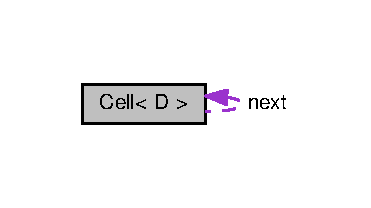
\includegraphics[width=178pt]{class_cell__coll__graph}
\end{center}
\end{figure}
\subsection*{Public Member Functions}
\begin{DoxyCompactItemize}
\item 
{\bf Cell} ()
\item 
{\bf Cell} (D $\ast$d, {\bf Cell} $\ast$c)
\item 
{\bfseries Cell} (const {\bf Cell} \&orig)\label{class_cell_a260a5d52d571c8d2f951d81df17154e2}

\end{DoxyCompactItemize}
\subsection*{Public Attributes}
\begin{DoxyCompactItemize}
\item 
{\bf Cell} $\ast$ {\bf next}\label{class_cell_a7e0e6c090f8aca70862c2dbc3257e3b9}

\begin{DoxyCompactList}\small\item\em Puntero que apunta a la celda siguiente. \end{DoxyCompactList}\item 
D $\ast$ {\bf data}\label{class_cell_ab8cc4d3059ef84a652eabc05b6c28f49}

\begin{DoxyCompactList}\small\item\em Puntero que apunta al dato almacenado en la celda. \end{DoxyCompactList}\end{DoxyCompactItemize}


\subsection{Detailed Description}
\subsubsection*{template$<$typename D$>$class Cell$<$ D $>$}

Plantilla de la clase Celda 

\subsection{Constructor \& Destructor Documentation}
\index{Cell@{Cell}!Cell@{Cell}}
\index{Cell@{Cell}!Cell@{Cell}}
\subsubsection[{Cell}]{\setlength{\rightskip}{0pt plus 5cm}template$<$typename D $>$ {\bf Cell}$<$ D $>$\-::{\bf Cell} (
\begin{DoxyParamCaption}
{}
\end{DoxyParamCaption}
)\hspace{0.3cm}{\ttfamily [inline]}}\label{class_cell_a742a2adf7fa420fa9cbe386a87b5c79b}
Constructor de la clase celda, sus atributos inician en nulo \index{Cell@{Cell}!Cell@{Cell}}
\index{Cell@{Cell}!Cell@{Cell}}
\subsubsection[{Cell}]{\setlength{\rightskip}{0pt plus 5cm}template$<$typename D $>$ {\bf Cell}$<$ D $>$\-::{\bf Cell} (
\begin{DoxyParamCaption}
\item[{D $\ast$}]{d, }
\item[{{\bf Cell}$<$ D $>$ $\ast$}]{c}
\end{DoxyParamCaption}
)\hspace{0.3cm}{\ttfamily [inline]}}\label{class_cell_aa8960323a8eeb23294419dd31349f18f}
Constructor de la clase celda, asigna a data y next, los valores recibidos como atributos 
\begin{DoxyParams}{Parameters}
{\em d} & puntero de tipo D \\
\hline
{\em c} & puntero de tipo \doxyref{Cell}{p.}{class_cell} \\
\hline
\end{DoxyParams}


The documentation for this class was generated from the following file\-:\begin{DoxyCompactItemize}
\item 
Cell.\-h\end{DoxyCompactItemize}

\hypertarget{class_list}{\section{Referencia de la plantilla de la Clase List$<$ D, P $>$}
\label{class_list}\index{List$<$ D, P $>$@{List$<$ D, P $>$}}
}


{\ttfamily \#include $<$List.\-h$>$}



Diagrama de herencias de List$<$ D, P $>$\nopagebreak
\begin{figure}[H]
\begin{center}
\leavevmode
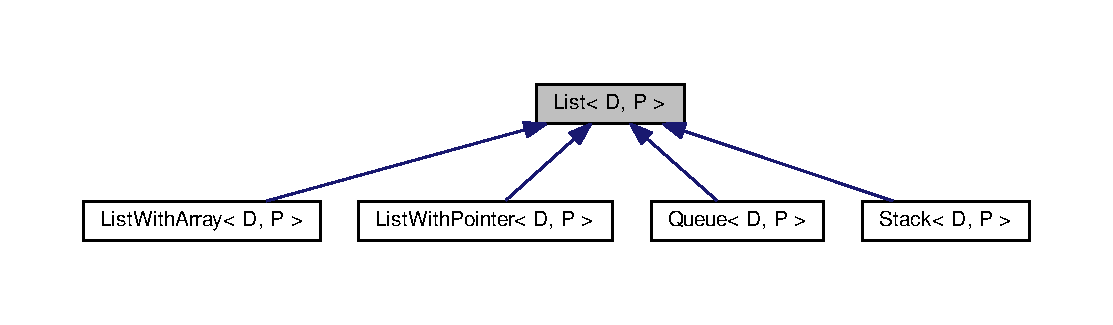
\includegraphics[width=202pt]{class_list__inherit__graph}
\end{center}
\end{figure}
\subsection*{Métodos públicos}
\begin{DoxyCompactItemize}
\item 
\hyperlink{class_list_a3deb54ab4f51c6c39aa4015f258b5812}{List} ()
\item 
\hyperlink{class_list_ad4d8108cecffb02dbc5e5e48691a0d43}{List} (int t)
\item 
\hyperlink{class_list_af8bcd7dae1bc30af2158075482c3d8d9}{List} (const \hyperlink{class_list}{List} \&orig)
\item 
virtual \hyperlink{class_list_a624593fb77847bf7ad4cacfba3442471}{$\sim$\-List} ()
\item 
virtual void \hyperlink{class_list_a01f588d87d47f8332928eca38f7b11bb}{insert} (D d)=0
\item 
virtual void \hyperlink{class_list_a14fc4e853102018df78db3899aa00d71}{remove} (D d)=0
\item 
virtual P \hyperlink{class_list_a2b40d6fffc7b2fb5138b648f52c839ee}{find} (D d)=0
\item 
virtual D \hyperlink{class_list_a5bd565e668247ae0691983227367cc88}{get} (P k)=0
\item 
virtual void \hyperlink{class_list_acb062aa988f4048498b30a2d845a311b}{assign} (P k, D d)=0
\item 
virtual void \hyperlink{class_list_ae3795939f27cf3e688cd470450e0c27a}{sort} ()=0
\item 
virtual int \hyperlink{class_list_af213bbcf13ee436a0f04cde66e337672}{get\-Size} ()=0
\item 
virtual void \hyperlink{class_list_a8b34931e187e7e6b86aad86510ce4f3b}{print\-List} ()=0
\item 
virtual P \hyperlink{class_list_a4ec3e88e176bb45bc49b030d1c8abb3f}{next} (P k)=0
\item 
virtual P \hyperlink{class_list_acc1831ae92a288345ef20cb29f3846b2}{prev} (P k)=0
\item 
virtual void \hyperlink{class_list_a24b4f177a70215980e81ef7b2981fa1e}{empty\-List} ()=0
\end{DoxyCompactItemize}


\subsection{Descripción detallada}
\subsubsection*{template$<$typename D, typename P$>$class List$<$ D, P $>$}

Plantilla de la clase \hyperlink{class_list}{List} 

\subsection{Documentación del constructor y destructor}
\hypertarget{class_list_a3deb54ab4f51c6c39aa4015f258b5812}{\index{List@{List}!List@{List}}
\index{List@{List}!List@{List}}
\subsubsection[{List}]{\setlength{\rightskip}{0pt plus 5cm}template$<$typename D, typename P$>$ {\bf List}$<$ D, P $>$\-::{\bf List} (
\begin{DoxyParamCaption}
{}
\end{DoxyParamCaption}
)\hspace{0.3cm}{\ttfamily [inline]}}}\label{class_list_a3deb54ab4f51c6c39aa4015f258b5812}
Constructor de la clase Lista sin atributos \hypertarget{class_list_ad4d8108cecffb02dbc5e5e48691a0d43}{\index{List@{List}!List@{List}}
\index{List@{List}!List@{List}}
\subsubsection[{List}]{\setlength{\rightskip}{0pt plus 5cm}template$<$typename D, typename P$>$ {\bf List}$<$ D, P $>$\-::{\bf List} (
\begin{DoxyParamCaption}
\item[{int}]{t}
\end{DoxyParamCaption}
)\hspace{0.3cm}{\ttfamily [inline]}}}\label{class_list_ad4d8108cecffb02dbc5e5e48691a0d43}
Constructor de la clase Lista. 
\begin{DoxyParams}{Parámetros}
{\em t} & tamaño de la lista \\
\hline
\end{DoxyParams}
\hypertarget{class_list_af8bcd7dae1bc30af2158075482c3d8d9}{\index{List@{List}!List@{List}}
\index{List@{List}!List@{List}}
\subsubsection[{List}]{\setlength{\rightskip}{0pt plus 5cm}template$<$typename D, typename P$>$ {\bf List}$<$ D, P $>$\-::{\bf List} (
\begin{DoxyParamCaption}
\item[{const {\bf List}$<$ D, P $>$ \&}]{orig}
\end{DoxyParamCaption}
)\hspace{0.3cm}{\ttfamily [inline]}}}\label{class_list_af8bcd7dae1bc30af2158075482c3d8d9}
Constructor por copia \hypertarget{class_list_a624593fb77847bf7ad4cacfba3442471}{\index{List@{List}!$\sim$\-List@{$\sim$\-List}}
\index{$\sim$\-List@{$\sim$\-List}!List@{List}}
\subsubsection[{$\sim$\-List}]{\setlength{\rightskip}{0pt plus 5cm}template$<$typename D, typename P$>$ virtual {\bf List}$<$ D, P $>$\-::$\sim${\bf List} (
\begin{DoxyParamCaption}
{}
\end{DoxyParamCaption}
)\hspace{0.3cm}{\ttfamily [inline]}, {\ttfamily [virtual]}}}\label{class_list_a624593fb77847bf7ad4cacfba3442471}
Destructor de la clase lista 

\subsection{Documentación de las funciones miembro}
\hypertarget{class_list_acb062aa988f4048498b30a2d845a311b}{\index{List@{List}!assign@{assign}}
\index{assign@{assign}!List@{List}}
\subsubsection[{assign}]{\setlength{\rightskip}{0pt plus 5cm}template$<$typename D, typename P$>$ virtual void {\bf List}$<$ D, P $>$\-::assign (
\begin{DoxyParamCaption}
\item[{P}]{k, }
\item[{D}]{d}
\end{DoxyParamCaption}
)\hspace{0.3cm}{\ttfamily [pure virtual]}}}\label{class_list_acb062aa988f4048498b30a2d845a311b}
Metodo virtual assign, asigna a una determinada posicion k, el valor d 
\begin{DoxyParams}{Parámetros}
{\em k} & dato tipo P, es una posicion o celda. \\
\hline
{\em d} & dado tipo D, que se quiere asignar a k \\
\hline
\end{DoxyParams}


Implementado en \hyperlink{class_list_with_pointer_aeaa834b22c4d7276a77ff29df3da7a30}{List\-With\-Pointer$<$ D, P $>$} y \hyperlink{class_list_with_pointer_aeaa834b22c4d7276a77ff29df3da7a30}{List\-With\-Pointer$<$ string, Cell$<$ string $>$ $\ast$ $>$}.

\hypertarget{class_list_a24b4f177a70215980e81ef7b2981fa1e}{\index{List@{List}!empty\-List@{empty\-List}}
\index{empty\-List@{empty\-List}!List@{List}}
\subsubsection[{empty\-List}]{\setlength{\rightskip}{0pt plus 5cm}template$<$typename D, typename P$>$ virtual void {\bf List}$<$ D, P $>$\-::empty\-List (
\begin{DoxyParamCaption}
{}
\end{DoxyParamCaption}
)\hspace{0.3cm}{\ttfamily [pure virtual]}}}\label{class_list_a24b4f177a70215980e81ef7b2981fa1e}
Metodo empty\-List, vacia la lista 

Implementado en \hyperlink{class_list_with_pointer_aec4f5374971962c79d397bbcd0080199}{List\-With\-Pointer$<$ D, P $>$} y \hyperlink{class_list_with_pointer_aec4f5374971962c79d397bbcd0080199}{List\-With\-Pointer$<$ string, Cell$<$ string $>$ $\ast$ $>$}.

\hypertarget{class_list_a2b40d6fffc7b2fb5138b648f52c839ee}{\index{List@{List}!find@{find}}
\index{find@{find}!List@{List}}
\subsubsection[{find}]{\setlength{\rightskip}{0pt plus 5cm}template$<$typename D, typename P$>$ virtual P {\bf List}$<$ D, P $>$\-::find (
\begin{DoxyParamCaption}
\item[{D}]{d}
\end{DoxyParamCaption}
)\hspace{0.3cm}{\ttfamily [pure virtual]}}}\label{class_list_a2b40d6fffc7b2fb5138b648f52c839ee}
Metodo virtual find, busca dentro de la lista el dato d. 
\begin{DoxyParams}{Parámetros}
{\em d} & dato tipo D que se desea encontrar. \\
\hline
\end{DoxyParams}
\begin{DoxyReturn}{Devuelve}
posicion o celda donde se encuentra el dato 
\end{DoxyReturn}


Implementado en \hyperlink{class_list_with_pointer_afeff8b963c197378553e2a3f73eaf66a}{List\-With\-Pointer$<$ D, P $>$} y \hyperlink{class_list_with_pointer_afeff8b963c197378553e2a3f73eaf66a}{List\-With\-Pointer$<$ string, Cell$<$ string $>$ $\ast$ $>$}.

\hypertarget{class_list_a5bd565e668247ae0691983227367cc88}{\index{List@{List}!get@{get}}
\index{get@{get}!List@{List}}
\subsubsection[{get}]{\setlength{\rightskip}{0pt plus 5cm}template$<$typename D, typename P$>$ virtual D {\bf List}$<$ D, P $>$\-::get (
\begin{DoxyParamCaption}
\item[{P}]{k}
\end{DoxyParamCaption}
)\hspace{0.3cm}{\ttfamily [pure virtual]}}}\label{class_list_a5bd565e668247ae0691983227367cc88}
Metodo virtual get, da el valor que se encuentra almacenado en la posicion k. 
\begin{DoxyParams}{Parámetros}
{\em k} & dato tipo P, es una posicion o celda. \\
\hline
\end{DoxyParams}
\begin{DoxyReturn}{Devuelve}
retorna el valor almacenado en k 
\end{DoxyReturn}


Implementado en \hyperlink{class_list_with_pointer_a0ff36c852334da8bc167356e636c1846}{List\-With\-Pointer$<$ D, P $>$} y \hyperlink{class_list_with_pointer_a0ff36c852334da8bc167356e636c1846}{List\-With\-Pointer$<$ string, Cell$<$ string $>$ $\ast$ $>$}.

\hypertarget{class_list_af213bbcf13ee436a0f04cde66e337672}{\index{List@{List}!get\-Size@{get\-Size}}
\index{get\-Size@{get\-Size}!List@{List}}
\subsubsection[{get\-Size}]{\setlength{\rightskip}{0pt plus 5cm}template$<$typename D, typename P$>$ virtual int {\bf List}$<$ D, P $>$\-::get\-Size (
\begin{DoxyParamCaption}
{}
\end{DoxyParamCaption}
)\hspace{0.3cm}{\ttfamily [pure virtual]}}}\label{class_list_af213bbcf13ee436a0f04cde66e337672}
Metodo virtual get\-Size, da el tamaño de la lista. \begin{DoxyReturn}{Devuelve}
el tamaño de la lista 
\end{DoxyReturn}


Implementado en \hyperlink{class_list_with_pointer_ac70c49b5703887fd867e90cdac3c706f}{List\-With\-Pointer$<$ D, P $>$} y \hyperlink{class_list_with_pointer_ac70c49b5703887fd867e90cdac3c706f}{List\-With\-Pointer$<$ string, Cell$<$ string $>$ $\ast$ $>$}.

\hypertarget{class_list_a01f588d87d47f8332928eca38f7b11bb}{\index{List@{List}!insert@{insert}}
\index{insert@{insert}!List@{List}}
\subsubsection[{insert}]{\setlength{\rightskip}{0pt plus 5cm}template$<$typename D, typename P$>$ virtual void {\bf List}$<$ D, P $>$\-::insert (
\begin{DoxyParamCaption}
\item[{D}]{d}
\end{DoxyParamCaption}
)\hspace{0.3cm}{\ttfamily [pure virtual]}}}\label{class_list_a01f588d87d47f8332928eca38f7b11bb}
Metodo virtual insert, agrega el dato d a la lista. 
\begin{DoxyParams}{Parámetros}
{\em d} & dato tipo D que se desea agregar a la lista \\
\hline
\end{DoxyParams}


Implementado en \hyperlink{class_list_with_pointer_a676e57683ade8e179e8eff5885f7309a}{List\-With\-Pointer$<$ D, P $>$} y \hyperlink{class_list_with_pointer_a676e57683ade8e179e8eff5885f7309a}{List\-With\-Pointer$<$ string, Cell$<$ string $>$ $\ast$ $>$}.

\hypertarget{class_list_a4ec3e88e176bb45bc49b030d1c8abb3f}{\index{List@{List}!next@{next}}
\index{next@{next}!List@{List}}
\subsubsection[{next}]{\setlength{\rightskip}{0pt plus 5cm}template$<$typename D, typename P$>$ virtual P {\bf List}$<$ D, P $>$\-::next (
\begin{DoxyParamCaption}
\item[{P}]{k}
\end{DoxyParamCaption}
)\hspace{0.3cm}{\ttfamily [pure virtual]}}}\label{class_list_a4ec3e88e176bb45bc49b030d1c8abb3f}
Metodo next, da la posicion o celda que le sigue a k 
\begin{DoxyParams}{Parámetros}
{\em k} & dato tipo P, es una posicion o celda. \\
\hline
\end{DoxyParams}
\begin{DoxyReturn}{Devuelve}
la posicion siguiente a k 
\end{DoxyReturn}


Implementado en \hyperlink{class_list_with_pointer_a518b5ee89e3ad32ae7cd4ddd5d4fa7e9}{List\-With\-Pointer$<$ D, P $>$} y \hyperlink{class_list_with_pointer_a518b5ee89e3ad32ae7cd4ddd5d4fa7e9}{List\-With\-Pointer$<$ string, Cell$<$ string $>$ $\ast$ $>$}.

\hypertarget{class_list_acc1831ae92a288345ef20cb29f3846b2}{\index{List@{List}!prev@{prev}}
\index{prev@{prev}!List@{List}}
\subsubsection[{prev}]{\setlength{\rightskip}{0pt plus 5cm}template$<$typename D, typename P$>$ virtual P {\bf List}$<$ D, P $>$\-::prev (
\begin{DoxyParamCaption}
\item[{P}]{k}
\end{DoxyParamCaption}
)\hspace{0.3cm}{\ttfamily [pure virtual]}}}\label{class_list_acc1831ae92a288345ef20cb29f3846b2}
Metodo next, retorna la posicion o celda que precede a k 
\begin{DoxyParams}{Parámetros}
{\em k} & dato tipo P, es una posicion o celda. \\
\hline
\end{DoxyParams}
\begin{DoxyReturn}{Devuelve}
la posicion previa a k 
\end{DoxyReturn}


Implementado en \hyperlink{class_list_with_pointer_a7242068fcc3a193f0f7e94517856e431}{List\-With\-Pointer$<$ D, P $>$} y \hyperlink{class_list_with_pointer_a7242068fcc3a193f0f7e94517856e431}{List\-With\-Pointer$<$ string, Cell$<$ string $>$ $\ast$ $>$}.

\hypertarget{class_list_a8b34931e187e7e6b86aad86510ce4f3b}{\index{List@{List}!print\-List@{print\-List}}
\index{print\-List@{print\-List}!List@{List}}
\subsubsection[{print\-List}]{\setlength{\rightskip}{0pt plus 5cm}template$<$typename D, typename P$>$ virtual void {\bf List}$<$ D, P $>$\-::print\-List (
\begin{DoxyParamCaption}
{}
\end{DoxyParamCaption}
)\hspace{0.3cm}{\ttfamily [pure virtual]}}}\label{class_list_a8b34931e187e7e6b86aad86510ce4f3b}
Metodo print\-List, imprime la lista 

Implementado en \hyperlink{class_list_with_pointer_a7079b5f1dbddb87a7e33ffc71ebb7b92}{List\-With\-Pointer$<$ D, P $>$} y \hyperlink{class_list_with_pointer_a7079b5f1dbddb87a7e33ffc71ebb7b92}{List\-With\-Pointer$<$ string, Cell$<$ string $>$ $\ast$ $>$}.

\hypertarget{class_list_a14fc4e853102018df78db3899aa00d71}{\index{List@{List}!remove@{remove}}
\index{remove@{remove}!List@{List}}
\subsubsection[{remove}]{\setlength{\rightskip}{0pt plus 5cm}template$<$typename D, typename P$>$ virtual void {\bf List}$<$ D, P $>$\-::remove (
\begin{DoxyParamCaption}
\item[{D}]{d}
\end{DoxyParamCaption}
)\hspace{0.3cm}{\ttfamily [pure virtual]}}}\label{class_list_a14fc4e853102018df78db3899aa00d71}
Metodo virtual remove , remueve el dato d de la lista, si este existe. 
\begin{DoxyParams}{Parámetros}
{\em d} & dato tipo D que se desea remover de la lista \\
\hline
\end{DoxyParams}


Implementado en \hyperlink{class_list_with_pointer_abcb151e95e9fffea7f9f7af593d8176f}{List\-With\-Pointer$<$ D, P $>$} y \hyperlink{class_list_with_pointer_abcb151e95e9fffea7f9f7af593d8176f}{List\-With\-Pointer$<$ string, Cell$<$ string $>$ $\ast$ $>$}.

\hypertarget{class_list_ae3795939f27cf3e688cd470450e0c27a}{\index{List@{List}!sort@{sort}}
\index{sort@{sort}!List@{List}}
\subsubsection[{sort}]{\setlength{\rightskip}{0pt plus 5cm}template$<$typename D, typename P$>$ virtual void {\bf List}$<$ D, P $>$\-::sort (
\begin{DoxyParamCaption}
{}
\end{DoxyParamCaption}
)\hspace{0.3cm}{\ttfamily [pure virtual]}}}\label{class_list_ae3795939f27cf3e688cd470450e0c27a}
Metodo virtual sort, ordena la lista 

Implementado en \hyperlink{class_list_with_pointer_aa46631b2da29895d1f767626fb591bc8}{List\-With\-Pointer$<$ D, P $>$} y \hyperlink{class_list_with_pointer_aa46631b2da29895d1f767626fb591bc8}{List\-With\-Pointer$<$ string, Cell$<$ string $>$ $\ast$ $>$}.



La documentación para esta clase fue generada a partir del siguiente fichero\-:\begin{DoxyCompactItemize}
\item 
List.\-h\end{DoxyCompactItemize}

\section{List\-With\-Array$<$ D, P $>$ Class Template Reference}
\label{class_list_with_array}\index{List\-With\-Array$<$ D, P $>$@{List\-With\-Array$<$ D, P $>$}}


Inheritance diagram for List\-With\-Array$<$ D, P $>$\-:\nopagebreak
\begin{figure}[H]
\begin{center}
\leavevmode
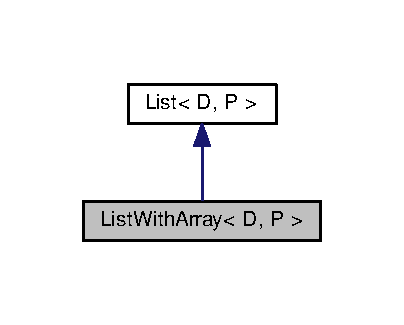
\includegraphics[width=194pt]{class_list_with_array__inherit__graph}
\end{center}
\end{figure}


Collaboration diagram for List\-With\-Array$<$ D, P $>$\-:\nopagebreak
\begin{figure}[H]
\begin{center}
\leavevmode
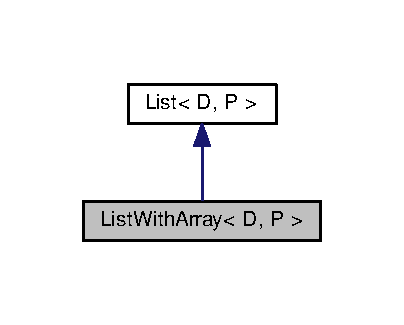
\includegraphics[width=194pt]{class_list_with_array__coll__graph}
\end{center}
\end{figure}
\subsection*{Public Member Functions}
\begin{DoxyCompactItemize}
\item 
{\bf List\-With\-Array} ()
\begin{DoxyCompactList}\small\item\em Constructor \doxyref{List\-With\-Array}{p.}{class_list_with_array}. \end{DoxyCompactList}\item 
{\bf List\-With\-Array} (int t)
\begin{DoxyCompactList}\small\item\em Constructor por copia de \doxyref{List\-With\-Array}{p.}{class_list_with_array}. \end{DoxyCompactList}\item 
{\bfseries List\-With\-Array} (const {\bf List\-With\-Array} \&orig)\label{class_list_with_array_a760ab3b39abb104e76a1fdbd2d303cc2}

\item 
{\bf $\sim$\-List\-With\-Array} ()\label{class_list_with_array_a1886482555430b0f3eb5ebe02cbb0c87}

\begin{DoxyCompactList}\small\item\em Destructor de la clase \doxyref{List\-With\-Array}{p.}{class_list_with_array}. \end{DoxyCompactList}\item 
void {\bf insert} (D d)
\begin{DoxyCompactList}\small\item\em Se inserta un elemento d a la lista. \end{DoxyCompactList}\item 
void {\bf remove} (D d)
\begin{DoxyCompactList}\small\item\em Metodo remove. \end{DoxyCompactList}\item 
P {\bf find} (D d)
\begin{DoxyCompactList}\small\item\em Metodo find. \end{DoxyCompactList}\item 
D {\bf get} (P k)
\begin{DoxyCompactList}\small\item\em Metodo get. \end{DoxyCompactList}\item 
void {\bf assign} (P k, D d)
\item 
void {\bf sort} ()
\begin{DoxyCompactList}\small\item\em Metodo Sort. \end{DoxyCompactList}\item 
int {\bf get\-Size} ()
\begin{DoxyCompactList}\small\item\em Metodo get\-Size. \end{DoxyCompactList}\item 
void {\bf print\-List} ()
\begin{DoxyCompactList}\small\item\em Metodo print\-List. \end{DoxyCompactList}\item 
P {\bf next} (P k)
\begin{DoxyCompactList}\small\item\em Metodo next. \end{DoxyCompactList}\item 
P {\bf prev} (P k)
\begin{DoxyCompactList}\small\item\em Metodo prev. \end{DoxyCompactList}\item 
void {\bf empty\-List} ()
\begin{DoxyCompactList}\small\item\em Metodo empty\-List. \end{DoxyCompactList}\end{DoxyCompactItemize}
\subsection*{Protected Attributes}
\begin{DoxyCompactItemize}
\item 
int {\bf n}\label{class_list_with_array_aa6b1712d5b006406885ee5c009d74800}

\begin{DoxyCompactList}\small\item\em Numero de elementos de la lista. \end{DoxyCompactList}\item 
int {\bf max\-Elements}\label{class_list_with_array_ae53e52b0fc76b833e247c1a00def10ff}

\begin{DoxyCompactList}\small\item\em Maxima cantidad de elementos que puede contener el arreglo. \end{DoxyCompactList}\item 
P {\bf last}\label{class_list_with_array_a269702c543590d3a63d5e00f0066dd9b}

\begin{DoxyCompactList}\small\item\em Ultimo posicion de la lista. \end{DoxyCompactList}\item 
D $\ast$ {\bf data}\label{class_list_with_array_a543b4698898dc963eac3ac6aa8f790ab}

\begin{DoxyCompactList}\small\item\em Puntero que apunda al contenido de un elemento de la lista. \end{DoxyCompactList}\end{DoxyCompactItemize}


\subsection{Constructor \& Destructor Documentation}
\index{List\-With\-Array@{List\-With\-Array}!List\-With\-Array@{List\-With\-Array}}
\index{List\-With\-Array@{List\-With\-Array}!ListWithArray@{List\-With\-Array}}
\subsubsection[{List\-With\-Array}]{\setlength{\rightskip}{0pt plus 5cm}template$<$typename D, typename P$>$ {\bf List\-With\-Array}$<$ D, P $>$\-::{\bf List\-With\-Array} (
\begin{DoxyParamCaption}
{}
\end{DoxyParamCaption}
)\hspace{0.3cm}{\ttfamily [inline]}}\label{class_list_with_array_a06f0e8035e9cc43aff4d32c46a00fcf0}


Constructor \doxyref{List\-With\-Array}{p.}{class_list_with_array}. 

Crea el objeto tipo \doxyref{List\-With\-Array}{p.}{class_list_with_array}. Se inicializan los atributos de la clase a un valor neutro. Se asigna nullptr a los punteros y 0 a la cantidad de elementos. \index{List\-With\-Array@{List\-With\-Array}!List\-With\-Array@{List\-With\-Array}}
\index{List\-With\-Array@{List\-With\-Array}!ListWithArray@{List\-With\-Array}}
\subsubsection[{List\-With\-Array}]{\setlength{\rightskip}{0pt plus 5cm}template$<$typename D, typename P$>$ {\bf List\-With\-Array}$<$ D, P $>$\-::{\bf List\-With\-Array} (
\begin{DoxyParamCaption}
\item[{int}]{t}
\end{DoxyParamCaption}
)\hspace{0.3cm}{\ttfamily [inline]}}\label{class_list_with_array_a3a6d11f203fb0f7e458672e85db26b03}


Constructor por copia de \doxyref{List\-With\-Array}{p.}{class_list_with_array}. 

Crea el objeto tipo \doxyref{List\-With\-Array}{p.}{class_list_with_array}. Se crea un arreglo de tamaño t y de tipo D. 
\begin{DoxyParams}{Parameters}
{\em t} & es la cantidad de elementos. \\
\hline
\end{DoxyParams}


\subsection{Member Function Documentation}
\index{List\-With\-Array@{List\-With\-Array}!assign@{assign}}
\index{assign@{assign}!ListWithArray@{List\-With\-Array}}
\subsubsection[{assign}]{\setlength{\rightskip}{0pt plus 5cm}template$<$typename D, typename P$>$ void {\bf List\-With\-Array}$<$ D, P $>$\-::assign (
\begin{DoxyParamCaption}
\item[{P}]{k, }
\item[{D}]{d}
\end{DoxyParamCaption}
)\hspace{0.3cm}{\ttfamily [inline]}, {\ttfamily [virtual]}}\label{class_list_with_array_a9dd1fd2337c6c8d437de71aae0e816c8}
Metodo virtual assign, asigna a una determinada posicion k, el valor d 
\begin{DoxyParams}{Parameters}
{\em k} & dato tipo P, es una posicion o celda. \\
\hline
{\em d} & dado tipo D, que se quiere asignar a k \\
\hline
\end{DoxyParams}


Implements {\bf List$<$ D, P $>$} \doxyref{}{p.}{class_list_acb062aa988f4048498b30a2d845a311b}.

\index{List\-With\-Array@{List\-With\-Array}!empty\-List@{empty\-List}}
\index{empty\-List@{empty\-List}!ListWithArray@{List\-With\-Array}}
\subsubsection[{empty\-List}]{\setlength{\rightskip}{0pt plus 5cm}template$<$typename D, typename P$>$ void {\bf List\-With\-Array}$<$ D, P $>$\-::empty\-List (
\begin{DoxyParamCaption}
{}
\end{DoxyParamCaption}
)\hspace{0.3cm}{\ttfamily [inline]}, {\ttfamily [virtual]}}\label{class_list_with_array_a2179e228f285cc29b46bd5d13ba0b4ed}


Metodo empty\-List. 

Este metodo vacia la pila. La cantidad de elementos se asigna como 0. 

Implements {\bf List$<$ D, P $>$} \doxyref{}{p.}{class_list_a24b4f177a70215980e81ef7b2981fa1e}.

\index{List\-With\-Array@{List\-With\-Array}!find@{find}}
\index{find@{find}!ListWithArray@{List\-With\-Array}}
\subsubsection[{find}]{\setlength{\rightskip}{0pt plus 5cm}template$<$typename D, typename P$>$ P {\bf List\-With\-Array}$<$ D, P $>$\-::find (
\begin{DoxyParamCaption}
\item[{D}]{d}
\end{DoxyParamCaption}
)\hspace{0.3cm}{\ttfamily [inline]}, {\ttfamily [virtual]}}\label{class_list_with_array_a9a054a6d407dc5cb39575739fe412fff}


Metodo find. 

Se busca un elemento d en la lista. Se recorre la lista y si se encuentra un elemento igual a d, se retorna un indice i que indica la posicion en el arreglo de este elemento. En caso de que no se encuentre se retorna -\/1. 
\begin{DoxyParams}{Parameters}
{\em d} & es el elemento del tipo D que se desea buscar en la lista. \\
\hline
\end{DoxyParams}


Implements {\bf List$<$ D, P $>$} \doxyref{}{p.}{class_list_a2b40d6fffc7b2fb5138b648f52c839ee}.

\index{List\-With\-Array@{List\-With\-Array}!get@{get}}
\index{get@{get}!ListWithArray@{List\-With\-Array}}
\subsubsection[{get}]{\setlength{\rightskip}{0pt plus 5cm}template$<$typename D, typename P$>$ D {\bf List\-With\-Array}$<$ D, P $>$\-::get (
\begin{DoxyParamCaption}
\item[{P}]{k}
\end{DoxyParamCaption}
)\hspace{0.3cm}{\ttfamily [inline]}, {\ttfamily [virtual]}}\label{class_list_with_array_a20cfc82811967bc2a77a6e43b9cebb46}


Metodo get. 

Retorna el contenido en el arreglo data, en la posicion k. \begin{DoxyReturn}{Returns}
k, indica el indice de la lista. 
\end{DoxyReturn}


Implements {\bf List$<$ D, P $>$} \doxyref{}{p.}{class_list_a5bd565e668247ae0691983227367cc88}.

\index{List\-With\-Array@{List\-With\-Array}!get\-Size@{get\-Size}}
\index{get\-Size@{get\-Size}!ListWithArray@{List\-With\-Array}}
\subsubsection[{get\-Size}]{\setlength{\rightskip}{0pt plus 5cm}template$<$typename D, typename P$>$ int {\bf List\-With\-Array}$<$ D, P $>$\-::get\-Size (
\begin{DoxyParamCaption}
{}
\end{DoxyParamCaption}
)\hspace{0.3cm}{\ttfamily [inline]}, {\ttfamily [virtual]}}\label{class_list_with_array_ae7a071bcdde9ddbf4c40a716f5a09434}


Metodo get\-Size. 

Retorna la cantidad de elementos de la lista \begin{DoxyReturn}{Returns}
n, es posible determinar el tamaño de la lista con el atributo n. 
\end{DoxyReturn}


Implements {\bf List$<$ D, P $>$} \doxyref{}{p.}{class_list_af213bbcf13ee436a0f04cde66e337672}.

\index{List\-With\-Array@{List\-With\-Array}!insert@{insert}}
\index{insert@{insert}!ListWithArray@{List\-With\-Array}}
\subsubsection[{insert}]{\setlength{\rightskip}{0pt plus 5cm}template$<$typename D, typename P$>$ void {\bf List\-With\-Array}$<$ D, P $>$\-::insert (
\begin{DoxyParamCaption}
\item[{D}]{d}
\end{DoxyParamCaption}
)\hspace{0.3cm}{\ttfamily [inline]}, {\ttfamily [virtual]}}\label{class_list_with_array_afa0b6d215c2cc1d3fe6b9b48d6b6917d}


Se inserta un elemento d a la lista. 

Se inserta el elemento de la siguiente forma. En caso de que la lista este vacia, se crea por defecto un arreglo de tamaño 10, donde se asigna 10 como la maxima cantidad de elementos de la lista, y se guarda d en el arreglo data en la posicion 0. En caso de que la lista no este vacia, y aun no alcance su maxima cantidad de elementos se guarda d en el arreglo data en la posicion last. En caso de que el arreglo este lleno, se crea un arreglo nuevo del doble de tamaño, se reajusta la maxima cantidad de elementos y ahora si es posible insertar el valor en la posicion last del arreglo data. 
\begin{DoxyParams}{Parameters}
{\em d} & es el elemento del tipo D que se desea ingresar en la lista. \\
\hline
\end{DoxyParams}


Implements {\bf List$<$ D, P $>$} \doxyref{}{p.}{class_list_a01f588d87d47f8332928eca38f7b11bb}.

\index{List\-With\-Array@{List\-With\-Array}!next@{next}}
\index{next@{next}!ListWithArray@{List\-With\-Array}}
\subsubsection[{next}]{\setlength{\rightskip}{0pt plus 5cm}template$<$typename D, typename P$>$ P {\bf List\-With\-Array}$<$ D, P $>$\-::next (
\begin{DoxyParamCaption}
\item[{P}]{k}
\end{DoxyParamCaption}
)\hspace{0.3cm}{\ttfamily [inline]}, {\ttfamily [virtual]}}\label{class_list_with_array_a125811011abb77c1b11e5150f4524fb1}


Metodo next. 

Este metodo es util para encontrar el elemento siguiente a otro elemento de la lista. \begin{DoxyReturn}{Returns}
retorna k+1 en caso de que el elemento k tenga un elemento siguiente. caso contrario retorna -\/1, lo que indica que no hay elemento siguiente. 
\end{DoxyReturn}


Implements {\bf List$<$ D, P $>$} \doxyref{}{p.}{class_list_a4ec3e88e176bb45bc49b030d1c8abb3f}.

\index{List\-With\-Array@{List\-With\-Array}!prev@{prev}}
\index{prev@{prev}!ListWithArray@{List\-With\-Array}}
\subsubsection[{prev}]{\setlength{\rightskip}{0pt plus 5cm}template$<$typename D, typename P$>$ P {\bf List\-With\-Array}$<$ D, P $>$\-::prev (
\begin{DoxyParamCaption}
\item[{P}]{k}
\end{DoxyParamCaption}
)\hspace{0.3cm}{\ttfamily [inline]}, {\ttfamily [virtual]}}\label{class_list_with_array_a72f0d74c4ae1fd4697088114db41d442}


Metodo prev. 

Este metodo es util para encontrar el elemento previo a otro elemento de la lista. \begin{DoxyReturn}{Returns}
retorna k-\/1 en caso de que el elemento k tenga un elemento previo. caso contrario retorna -\/1, lo que indica que no hay elemento previo. 
\end{DoxyReturn}


Implements {\bf List$<$ D, P $>$} \doxyref{}{p.}{class_list_acc1831ae92a288345ef20cb29f3846b2}.

\index{List\-With\-Array@{List\-With\-Array}!print\-List@{print\-List}}
\index{print\-List@{print\-List}!ListWithArray@{List\-With\-Array}}
\subsubsection[{print\-List}]{\setlength{\rightskip}{0pt plus 5cm}template$<$typename D, typename P$>$ void {\bf List\-With\-Array}$<$ D, P $>$\-::print\-List (
\begin{DoxyParamCaption}
{}
\end{DoxyParamCaption}
)\hspace{0.3cm}{\ttfamily [inline]}, {\ttfamily [virtual]}}\label{class_list_with_array_a515ea38cb40ba7b0c9df98825b2dd270}


Metodo print\-List. 

Imprime la lista. La lista se ve en pantalla en orden descendente, donde los elementos que se agregan a la lista van abajo. Se imprime c recorriendo todos sus elementos e imprimiendo el dato. A partir del metodo \doxyref{get()}{p.}{class_list_with_array_a20cfc82811967bc2a77a6e43b9cebb46}. 

Implements {\bf List$<$ D, P $>$} \doxyref{}{p.}{class_list_a8b34931e187e7e6b86aad86510ce4f3b}.

\index{List\-With\-Array@{List\-With\-Array}!remove@{remove}}
\index{remove@{remove}!ListWithArray@{List\-With\-Array}}
\subsubsection[{remove}]{\setlength{\rightskip}{0pt plus 5cm}template$<$typename D, typename P$>$ void {\bf List\-With\-Array}$<$ D, P $>$\-::remove (
\begin{DoxyParamCaption}
\item[{D}]{d}
\end{DoxyParamCaption}
)\hspace{0.3cm}{\ttfamily [inline]}, {\ttfamily [virtual]}}\label{class_list_with_array_aaa18e76fc128ca05151178d914901ec3}


Metodo remove. 

Se busca un elemento d en la lista. En caso de que exista lo remuevo reacomodando la lista. Disminuyo en 1 la cantidad de elementos y a last. 

Implements {\bf List$<$ D, P $>$} \doxyref{}{p.}{class_list_a14fc4e853102018df78db3899aa00d71}.

\index{List\-With\-Array@{List\-With\-Array}!sort@{sort}}
\index{sort@{sort}!ListWithArray@{List\-With\-Array}}
\subsubsection[{sort}]{\setlength{\rightskip}{0pt plus 5cm}template$<$typename D, typename P$>$ void {\bf List\-With\-Array}$<$ D, P $>$\-::sort (
\begin{DoxyParamCaption}
{}
\end{DoxyParamCaption}
)\hspace{0.3cm}{\ttfamily [inline]}, {\ttfamily [virtual]}}\label{class_list_with_array_a1a0ec4ab4a8fcb1a20568445ad892c9a}


Metodo Sort. 

Mediante el algoritmo de ordenamiento Bubble Sort, se ordenan los elementos de la lista en orden creciente. 

Implements {\bf List$<$ D, P $>$} \doxyref{}{p.}{class_list_ae3795939f27cf3e688cd470450e0c27a}.



The documentation for this class was generated from the following file\-:\begin{DoxyCompactItemize}
\item 
List\-With\-Array.\-h\end{DoxyCompactItemize}

\section{List\-With\-Pointer$<$ D, P $>$ Class Template Reference}
\label{class_list_with_pointer}\index{List\-With\-Pointer$<$ D, P $>$@{List\-With\-Pointer$<$ D, P $>$}}


{\ttfamily \#include $<$List\-With\-Pointer.\-h$>$}



Inheritance diagram for List\-With\-Pointer$<$ D, P $>$\-:\nopagebreak
\begin{figure}[H]
\begin{center}
\leavevmode
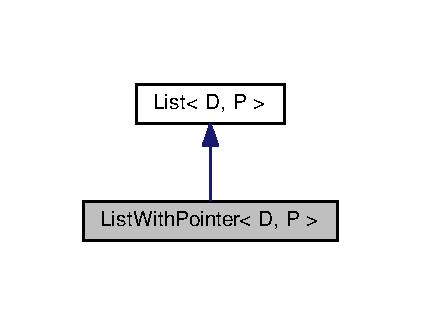
\includegraphics[width=202pt]{class_list_with_pointer__inherit__graph}
\end{center}
\end{figure}


Collaboration diagram for List\-With\-Pointer$<$ D, P $>$\-:\nopagebreak
\begin{figure}[H]
\begin{center}
\leavevmode
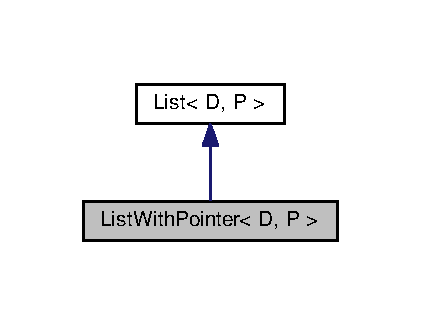
\includegraphics[width=202pt]{class_list_with_pointer__coll__graph}
\end{center}
\end{figure}
\subsection*{Public Member Functions}
\begin{DoxyCompactItemize}
\item 
{\bf List\-With\-Pointer} ()\label{class_list_with_pointer_a53b1284b13bf834bc5fc1eb27368a283}

\begin{DoxyCompactList}\small\item\em Constructor de la clase \doxyref{List\-With\-Pointer}{p.}{class_list_with_pointer}, los atributos first y null, son nulos y n es igual a cero. \end{DoxyCompactList}\item 
virtual {\bf $\sim$\-List\-With\-Pointer} ()\label{class_list_with_pointer_ac0567286c62e3521fa5130f95010e779}

\begin{DoxyCompactList}\small\item\em Destructor, elimina todos los elementos de la lista con \doxyref{empty\-List()}{p.}{class_list_with_pointer_aec4f5374971962c79d397bbcd0080199} \end{DoxyCompactList}\item 
void {\bf insert} (D d)
\begin{DoxyCompactList}\small\item\em Metodo insert. \end{DoxyCompactList}\item 
void {\bf remove} (D d)
\begin{DoxyCompactList}\small\item\em Metodo remove. \end{DoxyCompactList}\item 
P {\bf find} (D d)
\begin{DoxyCompactList}\small\item\em Metodo find. \end{DoxyCompactList}\item 
D {\bf get} (P k)
\begin{DoxyCompactList}\small\item\em Metodo get. \end{DoxyCompactList}\item 
void {\bf assign} (P k, D d)
\begin{DoxyCompactList}\small\item\em Metodo assign. \end{DoxyCompactList}\item 
void {\bf sort} ()
\begin{DoxyCompactList}\small\item\em Metodo sort. \end{DoxyCompactList}\item 
int {\bf get\-Size} ()
\begin{DoxyCompactList}\small\item\em Metodo get\-Size. \end{DoxyCompactList}\item 
void {\bf print\-List} ()
\begin{DoxyCompactList}\small\item\em Metodo print\-List. \end{DoxyCompactList}\item 
P {\bf next} (P k)
\begin{DoxyCompactList}\small\item\em Metodo next. \end{DoxyCompactList}\item 
P {\bf prev} (P k)
\begin{DoxyCompactList}\small\item\em Metodo previous. \end{DoxyCompactList}\item 
void {\bf empty\-List} ()
\begin{DoxyCompactList}\small\item\em Metodo empty\-List. \end{DoxyCompactList}\end{DoxyCompactItemize}
\subsection*{Public Attributes}
\begin{DoxyCompactItemize}
\item 
int {\bf n}\label{class_list_with_pointer_aac685c03cf811f155e2e0393a833ae33}

\begin{DoxyCompactList}\small\item\em Atributo de la clase que dice el tamaño de la lista. \end{DoxyCompactList}\item 
P {\bf first}\label{class_list_with_pointer_a10f9bcf73fcff6ca7fae28bec209bd20}

\begin{DoxyCompactList}\small\item\em Puntero de tipo celda que indica el primer elemento de la lista. \end{DoxyCompactList}\item 
P {\bf last}\label{class_list_with_pointer_aa4ff3f43dffeb524dc1cf3ac5dfdb415}

\begin{DoxyCompactList}\small\item\em Puntero de tipo celda que indica el ultimo elemento de la lista. \end{DoxyCompactList}\end{DoxyCompactItemize}


\subsection{Detailed Description}
\subsubsection*{template$<$typename D, typename P$>$class List\-With\-Pointer$<$ D, P $>$}

Plantilla de la clase Lista con Punteros, que hereda de la clase \doxyref{List}{p.}{class_list}. 

\subsection{Member Function Documentation}
\index{List\-With\-Pointer@{List\-With\-Pointer}!assign@{assign}}
\index{assign@{assign}!ListWithPointer@{List\-With\-Pointer}}
\subsubsection[{assign}]{\setlength{\rightskip}{0pt plus 5cm}template$<$typename D, typename P$>$ void {\bf List\-With\-Pointer}$<$ D, P $>$\-::assign (
\begin{DoxyParamCaption}
\item[{P}]{k, }
\item[{D}]{d}
\end{DoxyParamCaption}
)\hspace{0.3cm}{\ttfamily [inline]}, {\ttfamily [virtual]}}\label{class_list_with_pointer_aeaa834b22c4d7276a77ff29df3da7a30}


Metodo assign. 

Metodo para asignar a una celda existente en la lista, un valor especifico 
\begin{DoxyParams}{Parameters}
{\em k} & puntero tipo Celda. \\
\hline
{\em d} & dato tipo D, el cual se quiere asignar a la celda k. \\
\hline
\end{DoxyParams}


Implements {\bf List$<$ D, P $>$} \doxyref{}{p.}{class_list_acb062aa988f4048498b30a2d845a311b}.

\index{List\-With\-Pointer@{List\-With\-Pointer}!empty\-List@{empty\-List}}
\index{empty\-List@{empty\-List}!ListWithPointer@{List\-With\-Pointer}}
\subsubsection[{empty\-List}]{\setlength{\rightskip}{0pt plus 5cm}template$<$typename D, typename P$>$ void {\bf List\-With\-Pointer}$<$ D, P $>$\-::empty\-List (
\begin{DoxyParamCaption}
{}
\end{DoxyParamCaption}
)\hspace{0.3cm}{\ttfamily [inline]}, {\ttfamily [virtual]}}\label{class_list_with_pointer_aec4f5374971962c79d397bbcd0080199}


Metodo empty\-List. 

Metodo que se encarga de vaciar la lista. 

Implements {\bf List$<$ D, P $>$} \doxyref{}{p.}{class_list_a24b4f177a70215980e81ef7b2981fa1e}.

\index{List\-With\-Pointer@{List\-With\-Pointer}!find@{find}}
\index{find@{find}!ListWithPointer@{List\-With\-Pointer}}
\subsubsection[{find}]{\setlength{\rightskip}{0pt plus 5cm}template$<$typename D, typename P$>$ P {\bf List\-With\-Pointer}$<$ D, P $>$\-::find (
\begin{DoxyParamCaption}
\item[{D}]{d}
\end{DoxyParamCaption}
)\hspace{0.3cm}{\ttfamily [inline]}, {\ttfamily [virtual]}}\label{class_list_with_pointer_afeff8b963c197378553e2a3f73eaf66a}


Metodo find. 

Metodo de busqueda de un dato en la lista. 
\begin{DoxyParams}{Parameters}
{\em d} & dato tipo D que se desea buscar en la lista \\
\hline
\end{DoxyParams}
\begin{DoxyReturn}{Returns}
la celda en la cual se encuentra alojado el dato. 
\end{DoxyReturn}


Implements {\bf List$<$ D, P $>$} \doxyref{}{p.}{class_list_a2b40d6fffc7b2fb5138b648f52c839ee}.

\index{List\-With\-Pointer@{List\-With\-Pointer}!get@{get}}
\index{get@{get}!ListWithPointer@{List\-With\-Pointer}}
\subsubsection[{get}]{\setlength{\rightskip}{0pt plus 5cm}template$<$typename D, typename P$>$ D {\bf List\-With\-Pointer}$<$ D, P $>$\-::get (
\begin{DoxyParamCaption}
\item[{P}]{k}
\end{DoxyParamCaption}
)\hspace{0.3cm}{\ttfamily [inline]}, {\ttfamily [virtual]}}\label{class_list_with_pointer_a0ff36c852334da8bc167356e636c1846}


Metodo get. 

Metodo de obtencion del dato contenido en una celda 
\begin{DoxyParams}{Parameters}
{\em k} & puntero tipo Celda. \\
\hline
\end{DoxyParams}
\begin{DoxyReturn}{Returns}
Retorna el dato contenido en la celda. 
\end{DoxyReturn}


Implements {\bf List$<$ D, P $>$} \doxyref{}{p.}{class_list_a5bd565e668247ae0691983227367cc88}.

\index{List\-With\-Pointer@{List\-With\-Pointer}!get\-Size@{get\-Size}}
\index{get\-Size@{get\-Size}!ListWithPointer@{List\-With\-Pointer}}
\subsubsection[{get\-Size}]{\setlength{\rightskip}{0pt plus 5cm}template$<$typename D, typename P$>$ int {\bf List\-With\-Pointer}$<$ D, P $>$\-::get\-Size (
\begin{DoxyParamCaption}
{}
\end{DoxyParamCaption}
)\hspace{0.3cm}{\ttfamily [inline]}, {\ttfamily [virtual]}}\label{class_list_with_pointer_ac70c49b5703887fd867e90cdac3c706f}


Metodo get\-Size. 

Metodo que devuelve el tamaño de la lista \begin{DoxyReturn}{Returns}
tamaño. 
\end{DoxyReturn}


Implements {\bf List$<$ D, P $>$} \doxyref{}{p.}{class_list_af213bbcf13ee436a0f04cde66e337672}.

\index{List\-With\-Pointer@{List\-With\-Pointer}!insert@{insert}}
\index{insert@{insert}!ListWithPointer@{List\-With\-Pointer}}
\subsubsection[{insert}]{\setlength{\rightskip}{0pt plus 5cm}template$<$typename D, typename P$>$ void {\bf List\-With\-Pointer}$<$ D, P $>$\-::insert (
\begin{DoxyParamCaption}
\item[{D}]{d}
\end{DoxyParamCaption}
)\hspace{0.3cm}{\ttfamily [inline]}, {\ttfamily [virtual]}}\label{class_list_with_pointer_a676e57683ade8e179e8eff5885f7309a}


Metodo insert. 

Inserta elementos en la lista. Si la lista esta vacia, se crea la celda y se almacena el dato, los punteros first y last apuntan a dicha celda. De lo contrario, se crea la celda, se almacena el dato y se asigna el puntero last a la ultima celda agregada. Se hace la conexion entre la penultima celda y la ultima, mediante el atributo de la clase \doxyref{Cell}{p.}{class_cell}\-: next. Aumenta en uno a n. 
\begin{DoxyParams}{Parameters}
{\em d} & dato tipo D que se desea insertar en la lista. \\
\hline
{\em \doxyref{Cell}{p.}{class_cell}} & celda que se crea para almacenar el dato d. \\
\hline
\end{DoxyParams}


Implements {\bf List$<$ D, P $>$} \doxyref{}{p.}{class_list_a01f588d87d47f8332928eca38f7b11bb}.

\index{List\-With\-Pointer@{List\-With\-Pointer}!next@{next}}
\index{next@{next}!ListWithPointer@{List\-With\-Pointer}}
\subsubsection[{next}]{\setlength{\rightskip}{0pt plus 5cm}template$<$typename D, typename P$>$ P {\bf List\-With\-Pointer}$<$ D, P $>$\-::next (
\begin{DoxyParamCaption}
\item[{P}]{k}
\end{DoxyParamCaption}
)\hspace{0.3cm}{\ttfamily [inline]}, {\ttfamily [virtual]}}\label{class_list_with_pointer_a518b5ee89e3ad32ae7cd4ddd5d4fa7e9}


Metodo next. 

Metodo que dice la celda siguiente a una celda dada. 
\begin{DoxyParams}{Parameters}
{\em k} & puntero tipo celda. \\
\hline
\end{DoxyParams}
\begin{DoxyReturn}{Returns}
la celda siguiente a k. 
\end{DoxyReturn}


Implements {\bf List$<$ D, P $>$} \doxyref{}{p.}{class_list_a4ec3e88e176bb45bc49b030d1c8abb3f}.

\index{List\-With\-Pointer@{List\-With\-Pointer}!prev@{prev}}
\index{prev@{prev}!ListWithPointer@{List\-With\-Pointer}}
\subsubsection[{prev}]{\setlength{\rightskip}{0pt plus 5cm}template$<$typename D, typename P$>$ P {\bf List\-With\-Pointer}$<$ D, P $>$\-::prev (
\begin{DoxyParamCaption}
\item[{P}]{k}
\end{DoxyParamCaption}
)\hspace{0.3cm}{\ttfamily [inline]}, {\ttfamily [virtual]}}\label{class_list_with_pointer_a7242068fcc3a193f0f7e94517856e431}


Metodo previous. 

Metodo que dice la celda anterior a una celda dada. 
\begin{DoxyParams}{Parameters}
{\em k} & puntero tipo celda. \\
\hline
\end{DoxyParams}
\begin{DoxyReturn}{Returns}
la celda anterior a k. 
\end{DoxyReturn}


Implements {\bf List$<$ D, P $>$} \doxyref{}{p.}{class_list_acc1831ae92a288345ef20cb29f3846b2}.

\index{List\-With\-Pointer@{List\-With\-Pointer}!print\-List@{print\-List}}
\index{print\-List@{print\-List}!ListWithPointer@{List\-With\-Pointer}}
\subsubsection[{print\-List}]{\setlength{\rightskip}{0pt plus 5cm}template$<$typename D, typename P$>$ void {\bf List\-With\-Pointer}$<$ D, P $>$\-::print\-List (
\begin{DoxyParamCaption}
{}
\end{DoxyParamCaption}
)\hspace{0.3cm}{\ttfamily [inline]}, {\ttfamily [virtual]}}\label{class_list_with_pointer_a7079b5f1dbddb87a7e33ffc71ebb7b92}


Metodo print\-List. 

Metodo que imprime la lista. 

Implements {\bf List$<$ D, P $>$} \doxyref{}{p.}{class_list_a8b34931e187e7e6b86aad86510ce4f3b}.

\index{List\-With\-Pointer@{List\-With\-Pointer}!remove@{remove}}
\index{remove@{remove}!ListWithPointer@{List\-With\-Pointer}}
\subsubsection[{remove}]{\setlength{\rightskip}{0pt plus 5cm}template$<$typename D, typename P$>$ void {\bf List\-With\-Pointer}$<$ D, P $>$\-::remove (
\begin{DoxyParamCaption}
\item[{D}]{d}
\end{DoxyParamCaption}
)\hspace{0.3cm}{\ttfamily [inline]}, {\ttfamily [virtual]}}\label{class_list_with_pointer_abcb151e95e9fffea7f9f7af593d8176f}


Metodo remove. 

Remueve una celda de la lista. Se asegura que la lista no este vacia.\-De ser asi se crea un puntero temp tipo celda, que apunta a la celda que almacena el dato d. Si temp apunta a first, se cambia first a apuntar al siguiente valor de la lista. De lo contrario, se crea un puntero temp2 tipo celda que apunta al valor anterior a temp. Se realiza la conexion entre temp2, y la celda siguiente a temp. Se elimina temp. 
\begin{DoxyParams}{Parameters}
{\em d} & dato tipo D que se desea remover de la lista. \\
\hline
\end{DoxyParams}


Implements {\bf List$<$ D, P $>$} \doxyref{}{p.}{class_list_a14fc4e853102018df78db3899aa00d71}.

\index{List\-With\-Pointer@{List\-With\-Pointer}!sort@{sort}}
\index{sort@{sort}!ListWithPointer@{List\-With\-Pointer}}
\subsubsection[{sort}]{\setlength{\rightskip}{0pt plus 5cm}template$<$typename D, typename P$>$ void {\bf List\-With\-Pointer}$<$ D, P $>$\-::sort (
\begin{DoxyParamCaption}
{}
\end{DoxyParamCaption}
)\hspace{0.3cm}{\ttfamily [inline]}, {\ttfamily [virtual]}}\label{class_list_with_pointer_aa46631b2da29895d1f767626fb591bc8}


Metodo sort. 

Metodo para ordenar la lista de menor a mayor 

Implements {\bf List$<$ D, P $>$} \doxyref{}{p.}{class_list_ae3795939f27cf3e688cd470450e0c27a}.



The documentation for this class was generated from the following file\-:\begin{DoxyCompactItemize}
\item 
List\-With\-Pointer.\-h\end{DoxyCompactItemize}

\section{Queue$<$ D, P $>$ Class Template Reference}
\label{class_queue}\index{Queue$<$ D, P $>$@{Queue$<$ D, P $>$}}


{\ttfamily \#include $<$Queue.\-h$>$}



Inheritance diagram for Queue$<$ D, P $>$\-:
\nopagebreak
\begin{figure}[H]
\begin{center}
\leavevmode
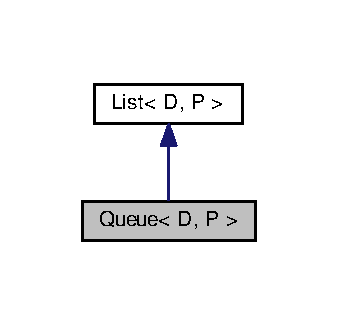
\includegraphics[width=162pt]{class_queue__inherit__graph}
\end{center}
\end{figure}


Collaboration diagram for Queue$<$ D, P $>$\-:
\nopagebreak
\begin{figure}[H]
\begin{center}
\leavevmode
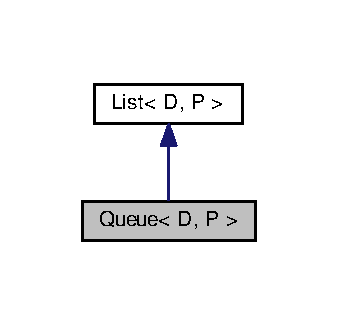
\includegraphics[width=162pt]{class_queue__coll__graph}
\end{center}
\end{figure}
\subsection*{Public Member Functions}
\begin{DoxyCompactItemize}
\item 
{\bf Queue} ()
\begin{DoxyCompactList}\small\item\em Constructor de la clase \doxyref{Queue}{p.}{class_queue}. \end{DoxyCompactList}\item 
virtual {\bf $\sim$\-Queue} ()
\begin{DoxyCompactList}\small\item\em Destructor de la clase \doxyref{Queue}{p.}{class_queue}. \end{DoxyCompactList}\item 
void {\bf insert} (D $\ast$d)
\begin{DoxyCompactList}\small\item\em Metodo de insercion de elementos a la cola. \end{DoxyCompactList}\item 
void {\bf remove} (D d)
\item 
P {\bf pop} ()
\item 
P {\bf find} (D d)
\item 
void {\bf assign} (P k, D d)
\item 
void {\bf sort} ()
\item 
int {\bf get\-Size} ()
\item 
void {\bf print\-List} ()
\item 
P {\bf next} (P k)
\item 
P {\bf prev} (P k)
\item 
D {\bf get} (P k)
\item 
void {\bf empty\-List} ()
\end{DoxyCompactItemize}
\subsection*{Public Attributes}
\begin{DoxyCompactItemize}
\item 
int {\bf n}
\begin{DoxyCompactList}\small\item\em Numero de elementos de la cola. \end{DoxyCompactList}\item 
P {\bf first}
\begin{DoxyCompactList}\small\item\em Puntero que apunta al primer elemento de la cola. \end{DoxyCompactList}\item 
P {\bf last}
\begin{DoxyCompactList}\small\item\em Puntero que apunta al último elemento de la cola. \end{DoxyCompactList}\end{DoxyCompactItemize}


\subsection{Detailed Description}
\subsubsection*{template$<$typename D, typename P$>$class Queue$<$ D, P $>$}

Plantilla de la clase Cola, que hereda de la clase Lista. 

\subsection{Constructor \& Destructor Documentation}
\index{Queue@{Queue}!Queue@{Queue}}
\index{Queue@{Queue}!Queue@{Queue}}
\subsubsection[{Queue}]{\setlength{\rightskip}{0pt plus 5cm}template$<$typename D, typename P$>$ {\bf Queue}$<$ D, P $>$\-::{\bf Queue} (
\begin{DoxyParamCaption}
{}
\end{DoxyParamCaption}
)\hspace{0.3cm}{\ttfamily [inline]}}\label{class_queue_aaecc8eba91905e5bda9752e0f85a150e}


Constructor de la clase \doxyref{Queue}{p.}{class_queue}. 

Constructor de una cola vacia \index{Queue@{Queue}!$\sim$\-Queue@{$\sim$\-Queue}}
\index{$\sim$\-Queue@{$\sim$\-Queue}!Queue@{Queue}}
\subsubsection[{$\sim$\-Queue}]{\setlength{\rightskip}{0pt plus 5cm}template$<$typename D, typename P$>$ virtual {\bf Queue}$<$ D, P $>$\-::$\sim${\bf Queue} (
\begin{DoxyParamCaption}
{}
\end{DoxyParamCaption}
)\hspace{0.3cm}{\ttfamily [inline]}, {\ttfamily [virtual]}}\label{class_queue_af88c0ebfc35932cdbbd75bae05e7a962}


Destructor de la clase \doxyref{Queue}{p.}{class_queue}. 

Llama al método empty\-List, para eliminar la cola. 

\subsection{Member Function Documentation}
\index{Queue@{Queue}!assign@{assign}}
\index{assign@{assign}!Queue@{Queue}}
\subsubsection[{assign}]{\setlength{\rightskip}{0pt plus 5cm}template$<$typename D, typename P$>$ void {\bf Queue}$<$ D, P $>$\-::assign (
\begin{DoxyParamCaption}
\item[{P}]{k, }
\item[{D}]{d}
\end{DoxyParamCaption}
)\hspace{0.3cm}{\ttfamily [inline]}, {\ttfamily [virtual]}}\label{class_queue_a81e1345ce465a07879f455fd1b6e086e}
Metodo assign, irrelevante para la cola 

Implements {\bf List$<$ D, P $>$} \doxyref{}{p.}{class_list_acb062aa988f4048498b30a2d845a311b}.

\index{Queue@{Queue}!empty\-List@{empty\-List}}
\index{empty\-List@{empty\-List}!Queue@{Queue}}
\subsubsection[{empty\-List}]{\setlength{\rightskip}{0pt plus 5cm}template$<$typename D, typename P$>$ void {\bf Queue}$<$ D, P $>$\-::empty\-List (
\begin{DoxyParamCaption}
{}
\end{DoxyParamCaption}
)\hspace{0.3cm}{\ttfamily [inline]}, {\ttfamily [virtual]}}\label{class_queue_a37e23ca9e4ac29be510833bf6b7f6638}
Metodo empty\-List, elimina todos los elementos pertenecientes a la cola. 

Implements {\bf List$<$ D, P $>$} \doxyref{}{p.}{class_list_a24b4f177a70215980e81ef7b2981fa1e}.

\index{Queue@{Queue}!find@{find}}
\index{find@{find}!Queue@{Queue}}
\subsubsection[{find}]{\setlength{\rightskip}{0pt plus 5cm}template$<$typename D, typename P$>$ P {\bf Queue}$<$ D, P $>$\-::find (
\begin{DoxyParamCaption}
\item[{D}]{d}
\end{DoxyParamCaption}
)\hspace{0.3cm}{\ttfamily [inline]}, {\ttfamily [virtual]}}\label{class_queue_a5c5ad7000d15506d3ec9c2ef6c8e6041}
Metodo find, irrelevante para la cola 

Implements {\bf List$<$ D, P $>$} \doxyref{}{p.}{class_list_a2b40d6fffc7b2fb5138b648f52c839ee}.

\index{Queue@{Queue}!get@{get}}
\index{get@{get}!Queue@{Queue}}
\subsubsection[{get}]{\setlength{\rightskip}{0pt plus 5cm}template$<$typename D, typename P$>$ D {\bf Queue}$<$ D, P $>$\-::get (
\begin{DoxyParamCaption}
\item[{P}]{k}
\end{DoxyParamCaption}
)\hspace{0.3cm}{\ttfamily [inline]}, {\ttfamily [virtual]}}\label{class_queue_a55cdbb6d999ef9a7a7afa5e39759701e}
Metodo get, irrelevante para la cola 

Implements {\bf List$<$ D, P $>$} \doxyref{}{p.}{class_list_a5bd565e668247ae0691983227367cc88}.

\index{Queue@{Queue}!get\-Size@{get\-Size}}
\index{get\-Size@{get\-Size}!Queue@{Queue}}
\subsubsection[{get\-Size}]{\setlength{\rightskip}{0pt plus 5cm}template$<$typename D, typename P$>$ int {\bf Queue}$<$ D, P $>$\-::get\-Size (
\begin{DoxyParamCaption}
{}
\end{DoxyParamCaption}
)\hspace{0.3cm}{\ttfamily [inline]}, {\ttfamily [virtual]}}\label{class_queue_ab2c7217e6737bf579493b321184a2db3}
Metodo get\-Size, da el tamaño de la cola. \begin{DoxyReturn}{Returns}
tamaño 
\end{DoxyReturn}


Implements {\bf List$<$ D, P $>$} \doxyref{}{p.}{class_list_af213bbcf13ee436a0f04cde66e337672}.

\index{Queue@{Queue}!insert@{insert}}
\index{insert@{insert}!Queue@{Queue}}
\subsubsection[{insert}]{\setlength{\rightskip}{0pt plus 5cm}template$<$typename D, typename P$>$ void {\bf Queue}$<$ D, P $>$\-::insert (
\begin{DoxyParamCaption}
\item[{D $\ast$}]{d}
\end{DoxyParamCaption}
)\hspace{0.3cm}{\ttfamily [inline]}, {\ttfamily [virtual]}}\label{class_queue_a3f3767b13bbd1a688dd13eb0fd8880c0}


Metodo de insercion de elementos a la cola. 

Dichos elementos solo pueden ser ingresados al final de la cola. Si la cola esta vacia, al insertar el elemento, este tendra los punteros first y last apuntando a él. De lo contrario, se crea la conexión entre el penúltimo elemento y el elemento agregado, y el puntero last apuntará a este elemento. 
\begin{DoxyParams}{Parameters}
{\em d} & dato tipo D que será ingresado a la cola. \\
\hline
\end{DoxyParams}


Implements {\bf List$<$ D, P $>$} \doxyref{}{p.}{class_list_a750822c0f61577bfb5297ea44aebe5a8}.

\index{Queue@{Queue}!next@{next}}
\index{next@{next}!Queue@{Queue}}
\subsubsection[{next}]{\setlength{\rightskip}{0pt plus 5cm}template$<$typename D, typename P$>$ P {\bf Queue}$<$ D, P $>$\-::next (
\begin{DoxyParamCaption}
\item[{P}]{k}
\end{DoxyParamCaption}
)\hspace{0.3cm}{\ttfamily [inline]}, {\ttfamily [virtual]}}\label{class_queue_aa4c9b83f260a172e1fffc389f354386f}
Metodo next, irrelevante para la cola 

Implements {\bf List$<$ D, P $>$} \doxyref{}{p.}{class_list_a4ec3e88e176bb45bc49b030d1c8abb3f}.

\index{Queue@{Queue}!pop@{pop}}
\index{pop@{pop}!Queue@{Queue}}
\subsubsection[{pop}]{\setlength{\rightskip}{0pt plus 5cm}template$<$typename D, typename P$>$ P {\bf Queue}$<$ D, P $>$\-::pop (
\begin{DoxyParamCaption}
{}
\end{DoxyParamCaption}
)\hspace{0.3cm}{\ttfamily [inline]}}\label{class_queue_aabf479754d981d43cebf7e8e68225881}
\index{Queue@{Queue}!prev@{prev}}
\index{prev@{prev}!Queue@{Queue}}
\subsubsection[{prev}]{\setlength{\rightskip}{0pt plus 5cm}template$<$typename D, typename P$>$ P {\bf Queue}$<$ D, P $>$\-::prev (
\begin{DoxyParamCaption}
\item[{P}]{k}
\end{DoxyParamCaption}
)\hspace{0.3cm}{\ttfamily [inline]}, {\ttfamily [virtual]}}\label{class_queue_adcb9a0e709ea65bc7e98f7e9cbae8a39}
Metodo prev, irrelevante para la cola 

Implements {\bf List$<$ D, P $>$} \doxyref{}{p.}{class_list_acc1831ae92a288345ef20cb29f3846b2}.

\index{Queue@{Queue}!print\-List@{print\-List}}
\index{print\-List@{print\-List}!Queue@{Queue}}
\subsubsection[{print\-List}]{\setlength{\rightskip}{0pt plus 5cm}template$<$typename D, typename P$>$ void {\bf Queue}$<$ D, P $>$\-::print\-List (
\begin{DoxyParamCaption}
{}
\end{DoxyParamCaption}
)\hspace{0.3cm}{\ttfamily [inline]}, {\ttfamily [virtual]}}\label{class_queue_aa461f8fb363f960a6e0eb34b18503eaa}
Metodo print\-List, imprime la cola 

Implements {\bf List$<$ D, P $>$} \doxyref{}{p.}{class_list_a8b34931e187e7e6b86aad86510ce4f3b}.

\index{Queue@{Queue}!remove@{remove}}
\index{remove@{remove}!Queue@{Queue}}
\subsubsection[{remove}]{\setlength{\rightskip}{0pt plus 5cm}template$<$typename D, typename P$>$ void {\bf Queue}$<$ D, P $>$\-::remove (
\begin{DoxyParamCaption}
\item[{D}]{d}
\end{DoxyParamCaption}
)\hspace{0.3cm}{\ttfamily [inline]}, {\ttfamily [virtual]}}\label{class_queue_a554993da9edb157443b0d956f11c8354}
Metodo que remueve el ultimo elemento de la cola. 
\begin{DoxyParams}{Parameters}
{\em d} & dato tipo D. Irrelevante para la cola. \\
\hline
\end{DoxyParams}


Implements {\bf List$<$ D, P $>$} \doxyref{}{p.}{class_list_a14fc4e853102018df78db3899aa00d71}.

\index{Queue@{Queue}!sort@{sort}}
\index{sort@{sort}!Queue@{Queue}}
\subsubsection[{sort}]{\setlength{\rightskip}{0pt plus 5cm}template$<$typename D, typename P$>$ void {\bf Queue}$<$ D, P $>$\-::sort (
\begin{DoxyParamCaption}
{}
\end{DoxyParamCaption}
)\hspace{0.3cm}{\ttfamily [inline]}, {\ttfamily [virtual]}}\label{class_queue_a896b0e1bcac0d660079eb838c1823446}
Metodo sort, irrelevante para la cola 

Implements {\bf List$<$ D, P $>$} \doxyref{}{p.}{class_list_ae3795939f27cf3e688cd470450e0c27a}.



\subsection{Member Data Documentation}
\index{Queue@{Queue}!first@{first}}
\index{first@{first}!Queue@{Queue}}
\subsubsection[{first}]{\setlength{\rightskip}{0pt plus 5cm}template$<$typename D, typename P$>$ P {\bf Queue}$<$ D, P $>$\-::first}\label{class_queue_a66d3f4dcd98ff256982192ccd4cbe1d4}


Puntero que apunta al primer elemento de la cola. 

\index{Queue@{Queue}!last@{last}}
\index{last@{last}!Queue@{Queue}}
\subsubsection[{last}]{\setlength{\rightskip}{0pt plus 5cm}template$<$typename D, typename P$>$ P {\bf Queue}$<$ D, P $>$\-::last}\label{class_queue_a8fa09b42d16c1fe9dea414b29ab9612f}


Puntero que apunta al último elemento de la cola. 

\index{Queue@{Queue}!n@{n}}
\index{n@{n}!Queue@{Queue}}
\subsubsection[{n}]{\setlength{\rightskip}{0pt plus 5cm}template$<$typename D, typename P$>$ int {\bf Queue}$<$ D, P $>$\-::n}\label{class_queue_a2b095618e827a9e728cb843bf4c0919e}


Numero de elementos de la cola. 



The documentation for this class was generated from the following file\-:\begin{DoxyCompactItemize}
\item 
{\bf Queue.\-h}\end{DoxyCompactItemize}

\section{Stack$<$ D, P $>$ Class Template Reference}
\label{class_stack}\index{Stack$<$ D, P $>$@{Stack$<$ D, P $>$}}


{\ttfamily \#include $<$Stack.\-h$>$}



Inheritance diagram for Stack$<$ D, P $>$\-:
\nopagebreak
\begin{figure}[H]
\begin{center}
\leavevmode
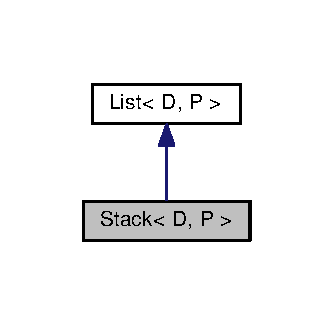
\includegraphics[width=160pt]{class_stack__inherit__graph}
\end{center}
\end{figure}


Collaboration diagram for Stack$<$ D, P $>$\-:
\nopagebreak
\begin{figure}[H]
\begin{center}
\leavevmode
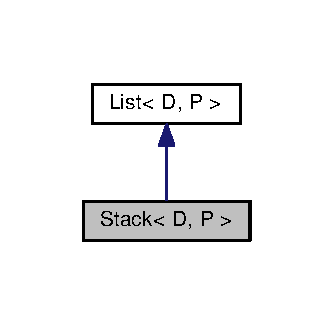
\includegraphics[width=160pt]{class_stack__coll__graph}
\end{center}
\end{figure}
\subsection*{Public Member Functions}
\begin{DoxyCompactItemize}
\item 
{\bf Stack} ()
\begin{DoxyCompactList}\small\item\em Constructor \doxyref{Stack}{p.}{class_stack}. \end{DoxyCompactList}\item 
void {\bf insert} (D $\ast$d)
\begin{DoxyCompactList}\small\item\em Metodo Insert. \end{DoxyCompactList}\item 
void {\bf remove} (D d)
\begin{DoxyCompactList}\small\item\em Metodo remove. \end{DoxyCompactList}\item 
void {\bf pop} ()
\item 
P {\bf find} (D d)
\item 
void {\bf assign} (P k, D d)
\item 
void {\bf sort} ()
\item 
int {\bf get\-Size} ()
\begin{DoxyCompactList}\small\item\em Metodo get\-Size. \end{DoxyCompactList}\item 
void {\bf print\-List} ()
\begin{DoxyCompactList}\small\item\em Metodo print\-List. \end{DoxyCompactList}\item 
P {\bf next} (P k)
\item 
P {\bf prev} (P k)
\begin{DoxyCompactList}\small\item\em Metodo prev. \end{DoxyCompactList}\item 
D {\bf get} (P k)
\item 
void {\bf empty\-List} ()
\end{DoxyCompactItemize}
\subsection*{Public Attributes}
\begin{DoxyCompactItemize}
\item 
int {\bf n}
\item 
P {\bf first}
\item 
P {\bf last}
\end{DoxyCompactItemize}


\subsection{Constructor \& Destructor Documentation}
\index{Stack@{Stack}!Stack@{Stack}}
\index{Stack@{Stack}!Stack@{Stack}}
\subsubsection[{Stack}]{\setlength{\rightskip}{0pt plus 5cm}template$<$typename D, typename P$>$ {\bf Stack}$<$ D, P $>$\-::{\bf Stack} (
\begin{DoxyParamCaption}
{}
\end{DoxyParamCaption}
)\hspace{0.3cm}{\ttfamily [inline]}}\label{class_stack_a6e0f84830cde41cb8d49818842d18d36}


Constructor \doxyref{Stack}{p.}{class_stack}. 

Crea el objeto tipo \doxyref{Stack}{p.}{class_stack}. 
\begin{DoxyParams}{Parameters}
{\em first} & es un puntero a la primera celda de la pila. \\
\hline
{\em last} & es un puntero a la ultima celda de la pila. \\
\hline
{\em n} & es la cantidad de elementos en la pila. \\
\hline
\end{DoxyParams}


\subsection{Member Function Documentation}
\index{Stack@{Stack}!assign@{assign}}
\index{assign@{assign}!Stack@{Stack}}
\subsubsection[{assign}]{\setlength{\rightskip}{0pt plus 5cm}template$<$typename D, typename P$>$ void {\bf Stack}$<$ D, P $>$\-::assign (
\begin{DoxyParamCaption}
\item[{P}]{k, }
\item[{D}]{d}
\end{DoxyParamCaption}
)\hspace{0.3cm}{\ttfamily [inline]}, {\ttfamily [virtual]}}\label{class_stack_ad36bacdff9f82a8718559606b46b145c}
Metodo virtual assign, asigna a una determinada posicion k, el valor d 
\begin{DoxyParams}{Parameters}
{\em k} & dato tipo P, es una posicion o celda. \\
\hline
{\em d} & dado tipo D, que se quiere asignar a k \\
\hline
\end{DoxyParams}


Implements {\bf List$<$ D, P $>$} \doxyref{}{p.}{class_list_acb062aa988f4048498b30a2d845a311b}.

\index{Stack@{Stack}!empty\-List@{empty\-List}}
\index{empty\-List@{empty\-List}!Stack@{Stack}}
\subsubsection[{empty\-List}]{\setlength{\rightskip}{0pt plus 5cm}template$<$typename D, typename P$>$ void {\bf Stack}$<$ D, P $>$\-::empty\-List (
\begin{DoxyParamCaption}
{}
\end{DoxyParamCaption}
)\hspace{0.3cm}{\ttfamily [inline]}, {\ttfamily [virtual]}}\label{class_stack_a8d4119c8d4be2822f20a525743aa296e}
Metodo empty\-List, vacia la lista 

Implements {\bf List$<$ D, P $>$} \doxyref{}{p.}{class_list_a24b4f177a70215980e81ef7b2981fa1e}.

\index{Stack@{Stack}!find@{find}}
\index{find@{find}!Stack@{Stack}}
\subsubsection[{find}]{\setlength{\rightskip}{0pt plus 5cm}template$<$typename D, typename P$>$ P {\bf Stack}$<$ D, P $>$\-::find (
\begin{DoxyParamCaption}
\item[{D}]{d}
\end{DoxyParamCaption}
)\hspace{0.3cm}{\ttfamily [inline]}, {\ttfamily [virtual]}}\label{class_stack_aa8a3a0b773900e44f641e3be9d9345da}
Metodo virtual find, busca dentro de la lista el dato d. 
\begin{DoxyParams}{Parameters}
{\em d} & dato tipo D que se desea encontrar. \\
\hline
\end{DoxyParams}
\begin{DoxyReturn}{Returns}
posicion o celda donde se encuentra el dato 
\end{DoxyReturn}


Implements {\bf List$<$ D, P $>$} \doxyref{}{p.}{class_list_a2b40d6fffc7b2fb5138b648f52c839ee}.

\index{Stack@{Stack}!get@{get}}
\index{get@{get}!Stack@{Stack}}
\subsubsection[{get}]{\setlength{\rightskip}{0pt plus 5cm}template$<$typename D, typename P$>$ D {\bf Stack}$<$ D, P $>$\-::get (
\begin{DoxyParamCaption}
\item[{P}]{k}
\end{DoxyParamCaption}
)\hspace{0.3cm}{\ttfamily [inline]}, {\ttfamily [virtual]}}\label{class_stack_a64eaffbf031ad032772e802ec88378df}
Metodo virtual get, da el valor que se encuentra almacenado en la posicion k. 
\begin{DoxyParams}{Parameters}
{\em k} & dato tipo P, es una posicion o celda. \\
\hline
\end{DoxyParams}
\begin{DoxyReturn}{Returns}
retorna el valor almacenado en k 
\end{DoxyReturn}


Implements {\bf List$<$ D, P $>$} \doxyref{}{p.}{class_list_a5bd565e668247ae0691983227367cc88}.

\index{Stack@{Stack}!get\-Size@{get\-Size}}
\index{get\-Size@{get\-Size}!Stack@{Stack}}
\subsubsection[{get\-Size}]{\setlength{\rightskip}{0pt plus 5cm}template$<$typename D, typename P$>$ int {\bf Stack}$<$ D, P $>$\-::get\-Size (
\begin{DoxyParamCaption}
{}
\end{DoxyParamCaption}
)\hspace{0.3cm}{\ttfamily [inline]}, {\ttfamily [virtual]}}\label{class_stack_a74fc7e5921dfb247f9ad7052c3c4297a}


Metodo get\-Size. 

Retorna la cantidad de elementos de la pila. \begin{DoxyReturn}{Returns}
n, es posible determinar el tamaño de la pila con el atributo n. 
\end{DoxyReturn}


Implements {\bf List$<$ D, P $>$} \doxyref{}{p.}{class_list_af213bbcf13ee436a0f04cde66e337672}.

\index{Stack@{Stack}!insert@{insert}}
\index{insert@{insert}!Stack@{Stack}}
\subsubsection[{insert}]{\setlength{\rightskip}{0pt plus 5cm}template$<$typename D, typename P$>$ void {\bf Stack}$<$ D, P $>$\-::insert (
\begin{DoxyParamCaption}
\item[{D $\ast$}]{d}
\end{DoxyParamCaption}
)\hspace{0.3cm}{\ttfamily [inline]}, {\ttfamily [virtual]}}\label{class_stack_afed02ed90b717dc8e34daf02e2d3b586}


Metodo Insert. 

Inserta un elemento a la pila. Se crea un objeto newest tipo celda, que almacena al dato d. En caso de que la pila este vacia, se almacena esta celda creada en los punteros last y first . En caso de que la pila no este vacia, se realiza la coneccion de manera que ahora la ultima celda se convierta en la penultima(apuntando a la ultima). Se suma 1 a la cantidad de elementos. 
\begin{DoxyParams}{Parameters}
{\em d} & es un dato tipo D que se desea insertar en la pila. \\
\hline
{\em newest} & es un objeto tipo P. \\
\hline
\end{DoxyParams}


Implements {\bf List$<$ D, P $>$} \doxyref{}{p.}{class_list_a750822c0f61577bfb5297ea44aebe5a8}.

\index{Stack@{Stack}!next@{next}}
\index{next@{next}!Stack@{Stack}}
\subsubsection[{next}]{\setlength{\rightskip}{0pt plus 5cm}template$<$typename D, typename P$>$ P {\bf Stack}$<$ D, P $>$\-::next (
\begin{DoxyParamCaption}
\item[{P}]{k}
\end{DoxyParamCaption}
)\hspace{0.3cm}{\ttfamily [inline]}, {\ttfamily [virtual]}}\label{class_stack_ab7f8f7e4ab10c00769c1debc5391fc17}
Metodo next, da la posicion o celda que le sigue a k 
\begin{DoxyParams}{Parameters}
{\em k} & dato tipo P, es una posicion o celda. \\
\hline
\end{DoxyParams}
\begin{DoxyReturn}{Returns}
la posicion siguiente a k 
\end{DoxyReturn}


Implements {\bf List$<$ D, P $>$} \doxyref{}{p.}{class_list_a4ec3e88e176bb45bc49b030d1c8abb3f}.

\index{Stack@{Stack}!pop@{pop}}
\index{pop@{pop}!Stack@{Stack}}
\subsubsection[{pop}]{\setlength{\rightskip}{0pt plus 5cm}template$<$typename D, typename P$>$ void {\bf Stack}$<$ D, P $>$\-::pop (
\begin{DoxyParamCaption}
{}
\end{DoxyParamCaption}
)\hspace{0.3cm}{\ttfamily [inline]}}\label{class_stack_a9b465ba5e1c0be277775755dd680e52d}
\index{Stack@{Stack}!prev@{prev}}
\index{prev@{prev}!Stack@{Stack}}
\subsubsection[{prev}]{\setlength{\rightskip}{0pt plus 5cm}template$<$typename D, typename P$>$ P {\bf Stack}$<$ D, P $>$\-::prev (
\begin{DoxyParamCaption}
\item[{P}]{k}
\end{DoxyParamCaption}
)\hspace{0.3cm}{\ttfamily [inline]}, {\ttfamily [virtual]}}\label{class_stack_a0c0b55f72c9249bfb9252bce1a93458d}


Metodo prev. 

Para una pila este metodo no tiene sentido, sin embargo es util para otros metodos de la clase. Este metodo recibe un puntero a un objeto tipo \doxyref{Cell}{p.}{class_cell}, y recorre toda la pila(tal como una lista), buscando que celda apunta a la celda indicada, a partir del atributo next. 
\begin{DoxyParams}{Parameters}
{\em k} & es un puntero a un objeto tipo \doxyref{Cell}{p.}{class_cell}. \\
\hline
\end{DoxyParams}
\begin{DoxyReturn}{Returns}
retorna un puntero a la celda previa si se encontro, caso contrario retorna un nullptr 
\end{DoxyReturn}


Implements {\bf List$<$ D, P $>$} \doxyref{}{p.}{class_list_acc1831ae92a288345ef20cb29f3846b2}.

\index{Stack@{Stack}!print\-List@{print\-List}}
\index{print\-List@{print\-List}!Stack@{Stack}}
\subsubsection[{print\-List}]{\setlength{\rightskip}{0pt plus 5cm}template$<$typename D, typename P$>$ void {\bf Stack}$<$ D, P $>$\-::print\-List (
\begin{DoxyParamCaption}
{}
\end{DoxyParamCaption}
)\hspace{0.3cm}{\ttfamily [inline]}, {\ttfamily [virtual]}}\label{class_stack_a89b9967c15c83fe7c257a42e49725881}


Metodo print\-List. 

Imprime la pila. La pila se ve en pantalla en orden descendente, donde los elementos que se agregan a la pila van abajo. Y por lo tanto es de abajo que se tienen que extraer los valores. Se imprime como si fuese una lista, recorriendo todos sus elementos e imprimiendo el dato correspondiente a cada elemento. 

Implements {\bf List$<$ D, P $>$} \doxyref{}{p.}{class_list_a8b34931e187e7e6b86aad86510ce4f3b}.

\index{Stack@{Stack}!remove@{remove}}
\index{remove@{remove}!Stack@{Stack}}
\subsubsection[{remove}]{\setlength{\rightskip}{0pt plus 5cm}template$<$typename D, typename P$>$ void {\bf Stack}$<$ D, P $>$\-::remove (
\begin{DoxyParamCaption}
\item[{D}]{d}
\end{DoxyParamCaption}
)\hspace{0.3cm}{\ttfamily [inline]}, {\ttfamily [virtual]}}\label{class_stack_a55637a6d0aed4283776ce2d159c3a58b}


Metodo remove. 

Remueve un elemento de la pila. Al ser una pila, se sigue un orden L\-I\-F\-O(\-Last In First Out) Basicamente se asigna la penultima posicion de la pila como la ultima, descartando el elemento que ingreso a la pila mas recientemente. Se resta 1 a la cantidad de elementos. 

Implements {\bf List$<$ D, P $>$} \doxyref{}{p.}{class_list_a14fc4e853102018df78db3899aa00d71}.

\index{Stack@{Stack}!sort@{sort}}
\index{sort@{sort}!Stack@{Stack}}
\subsubsection[{sort}]{\setlength{\rightskip}{0pt plus 5cm}template$<$typename D, typename P$>$ void {\bf Stack}$<$ D, P $>$\-::sort (
\begin{DoxyParamCaption}
{}
\end{DoxyParamCaption}
)\hspace{0.3cm}{\ttfamily [inline]}, {\ttfamily [virtual]}}\label{class_stack_a75261d2340f1f7b5e61b3770c0550982}
Metodo virtual sort, ordena la lista 

Implements {\bf List$<$ D, P $>$} \doxyref{}{p.}{class_list_ae3795939f27cf3e688cd470450e0c27a}.



\subsection{Member Data Documentation}
\index{Stack@{Stack}!first@{first}}
\index{first@{first}!Stack@{Stack}}
\subsubsection[{first}]{\setlength{\rightskip}{0pt plus 5cm}template$<$typename D, typename P$>$ P {\bf Stack}$<$ D, P $>$\-::first}\label{class_stack_a2678111341d8fbcf7a5727334051fe26}
\index{Stack@{Stack}!last@{last}}
\index{last@{last}!Stack@{Stack}}
\subsubsection[{last}]{\setlength{\rightskip}{0pt plus 5cm}template$<$typename D, typename P$>$ P {\bf Stack}$<$ D, P $>$\-::last}\label{class_stack_ad8eba32e315256e8af67f0383c8f9576}
\index{Stack@{Stack}!n@{n}}
\index{n@{n}!Stack@{Stack}}
\subsubsection[{n}]{\setlength{\rightskip}{0pt plus 5cm}template$<$typename D, typename P$>$ int {\bf Stack}$<$ D, P $>$\-::n}\label{class_stack_a640915a5eb039f4b13945b7fde167e17}


The documentation for this class was generated from the following file\-:\begin{DoxyCompactItemize}
\item 
{\bf Stack.\-h}\end{DoxyCompactItemize}

%--- End generated contents ---

% Index
\newpage
\phantomsection
\addcontentsline{toc}{chapter}{Index}
\printindex

\end{document}
